\documentclass{pgnotes}

\title{Energy}

\begin{document}

\maketitle

\section{Reducing IT power}

\subsection{Hardware}

\begin{itemize}
\item Turning off (and removing) unused / zombie servers.
\item Apply available power management settings on server hardware.
\item Replace hardware like-for-like with newer energy-efficient equipment
\end{itemize}


\subsection{Consolidation}
\label{sec:consolidation}

\begin{enumerate}
\item Using a smaller number of servers to provide required services
\item Replacement of multiple physical servers with virtual servers on fewer energy-efficient physical hosts.
\item Use of containers and other technologies to provide a ``halfway house'' between running multiple services on one server vs full virtualisation.
\end{enumerate}

\subsection{Migration}

Depending on business needs, certain workloads may be better served by migrating them to virtual servers provisioned on a cloud environment. 

\section{Equipment replacement}

Infrastructure equipment replacement carries high capital costs.
Seek:
\begin{itemize}
\item UPS with optimised efficiency.
\item Cooling system with optimal COP, EER metrics. 
\end{itemize}
These calculations would need to consider the characteristics of the equipment in varying conditions: e.g. part-load and seasonal.

\section{Containment}
\label{sec:containment}

See \citep{rasmussen:2017:the-different} for full details.

\subsection{Air mixing}

There are two key air streams in a data centre:
\begin{description}
\item[Cold supply air] from the CRAC / CRAH unit outlet on way to inlets of servers.
\item[Hot return air] from servers and other IT equipement exhaust outlets to inlets of CRAC/CRAHs.
\end{description}

We want servers to get coldest possible air.
Therefore all air should come from the cooling unit.
There should be no ``leakage'' of hot air back to the inlets of servers. 

Cooling units work best if they take in the hottest air in the room and cool it down.
The greater the differential between the hot return air and the ambient temperature, the better the cooling performance will be. 
Efficiency seriously hampered if CRACs pull in already cold air.

\begin{figure}[htbp]
  \centering
  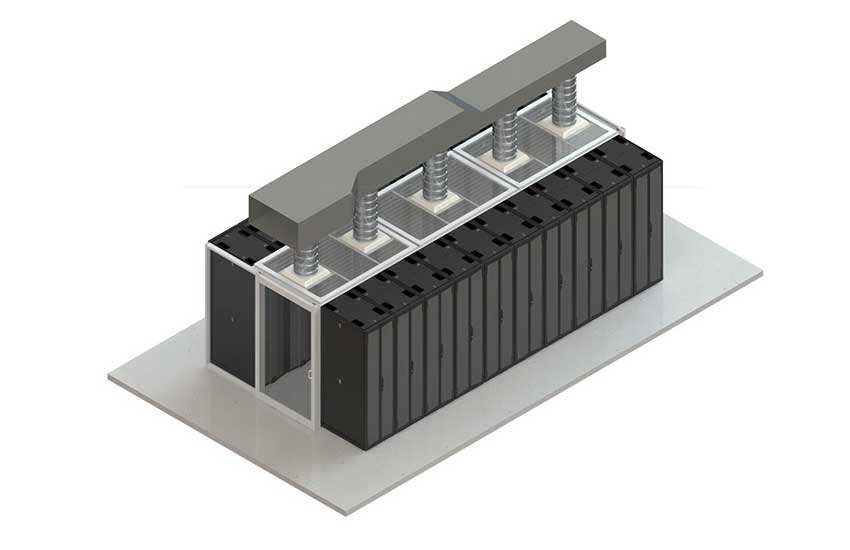
\includegraphics[width=0.75\linewidth]{containment_photo_subzero}
  \caption{Containment (Subzero Engineering)}
  \label{fig:containment-system}
\end{figure}

\subsection{Supply / return methods}

\begin{description}
\item[Flooded] air is supplied / removed from the room. 
\item[Targeted] air is supplied / removed within \SI{3}{\metre} the inlet / exhaust of the IT equipment. 
\item[Contained] supply / return systems completely enclose the relevant airflow to prevent mixing supply and return air streams. 
\end{description}

Containment is possible in both raised-floor and solid-floor environments.

\subsection{Hot / cold aisle}

As a minimum, we \textbf{must} be using hot / cold aisle arrangements, regardless of how small our data centre environment is!

A commonly encountered example is the targeted supply from raised floor with flooded return to CRAC as seen in \autoref{fig:hot-cold-aisle-airflow}. 

\begin{figure}[htbp]
  \centering
  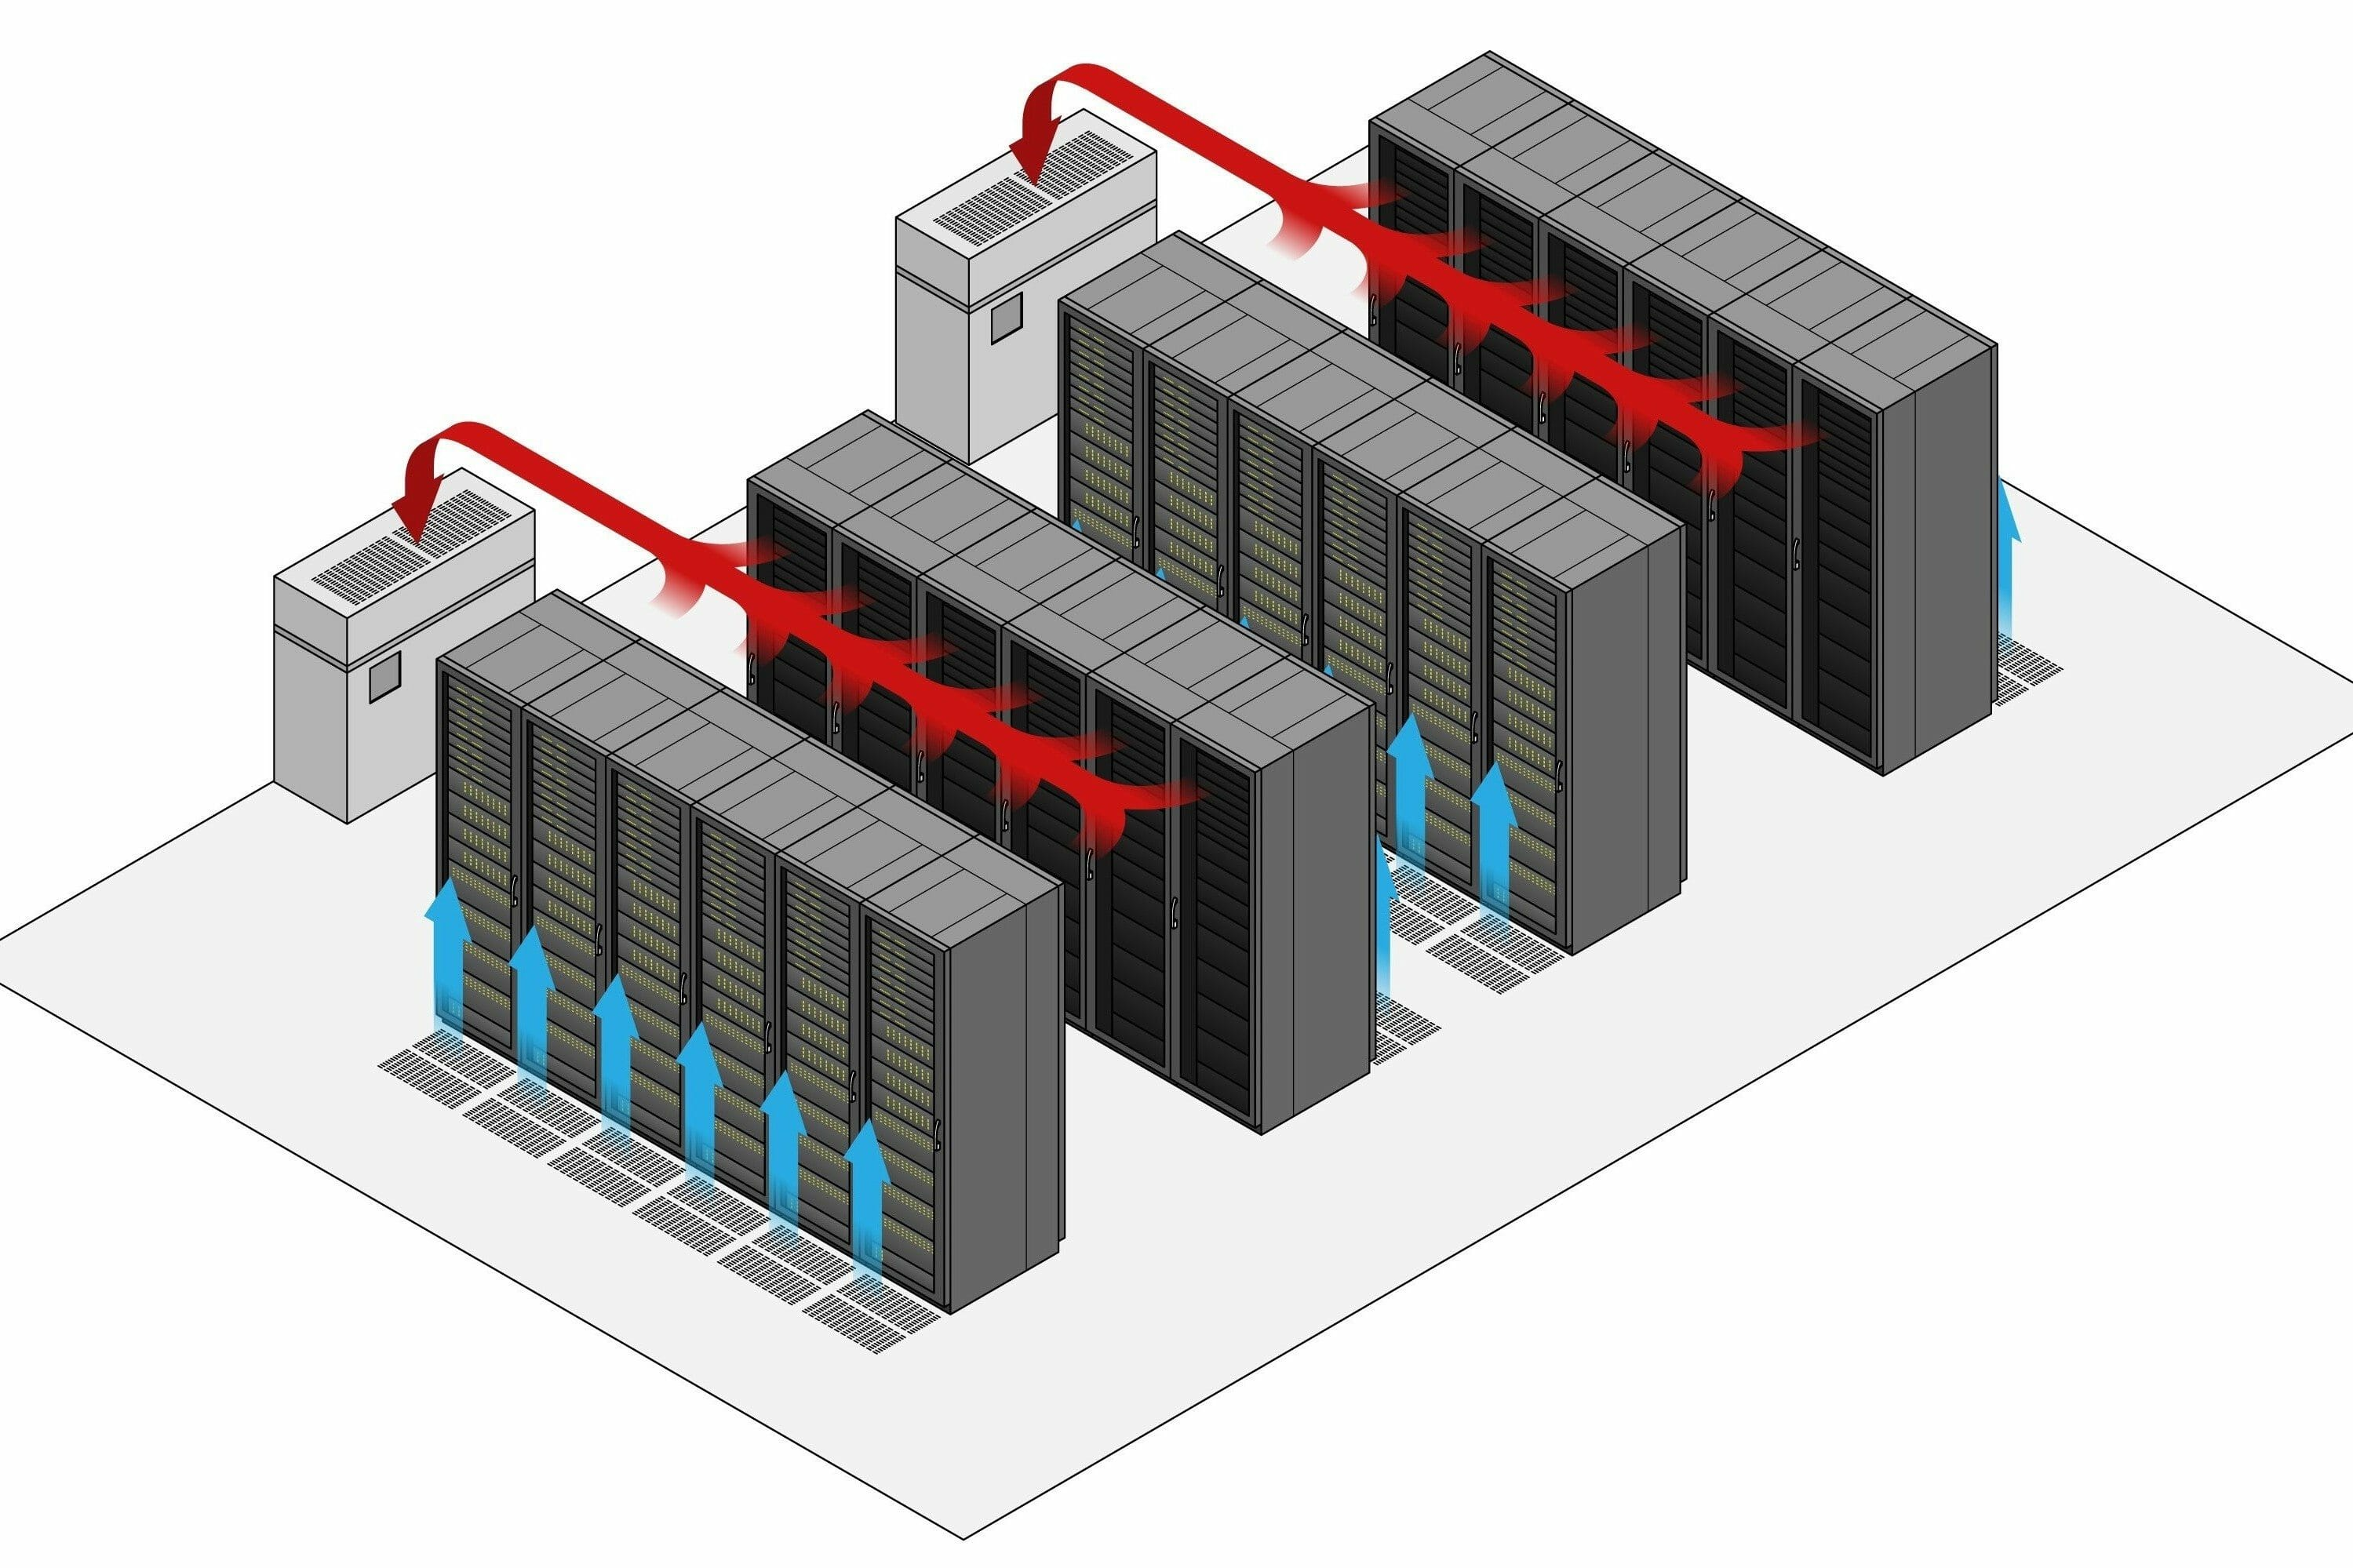
\includegraphics[width=0.75\linewidth]{dc_airflow}
  \caption{Hot/cold aisle airflow (Upsite.com)}
  \label{fig:hot-cold-aisle-airflow}
\end{figure}

%\subsection{Hot aisle containment}

%\subsection{Cold aisle containment}

\section{Economisation}
\label{sec:economisation}

Economisation aims to reduce the number of hours the refrigeration system must be in operation.
There are many ways to do this, with the principal methods detailed in \citet{niemann:2011:economizer}.

\begin{figure}[htbp]
  \centering
  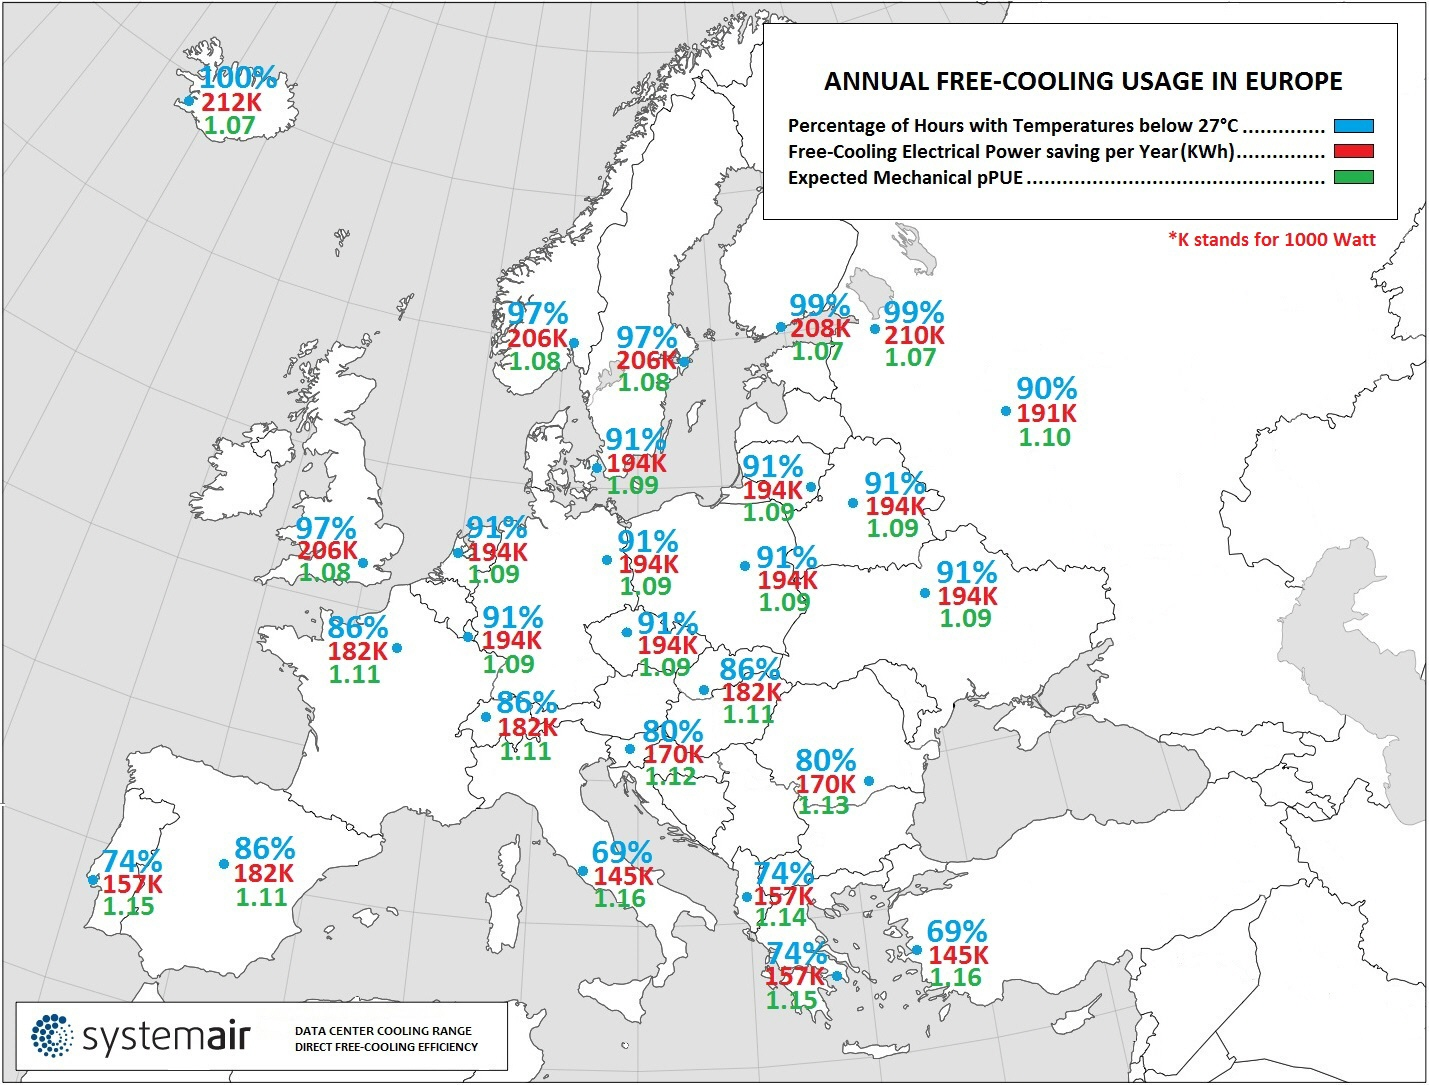
\includegraphics[width=0.75\linewidth]{free_cooling_europe_map_systemair}
  \caption{Direct free cooling map of Europe (SystemAir)}
  \label{fig:direct-free-cooling-map-europe}
\end{figure}


Some common configurations often seen in smaller environments are: 

\subsection{Direct airside economisation}

Direct airside economisation is normally found in conjunction with Air-Cooled DX CRACs but can be employed with any cooling system.
The idea is simple: when the outdoor air is cold enough, it is blown directly into the data centre.
\begin{itemize}
\item Simple solution with no additional plumbing needed.
\end{itemize}

Key requirements are:
\begin{itemize}
\item Outdoor air must be free of dust and pollutants.
\item Outdoor air should be of suitable humidity.
\item CRAC must be positioned to permit ducting to outside.
\end{itemize}


\subsection{Glycol/Water-based DX free cooling}

Glycol-cooled DX and Water-cooled DX CRACs can have an additional coil fitted within the case.
When the ambient temperature outside is low enough, the compressor can be shut down and a diverter valve sends water from the dry cooler / cooling tower outdoors to the economiser coil.

\begin{figure}[htbp]
  \centering
  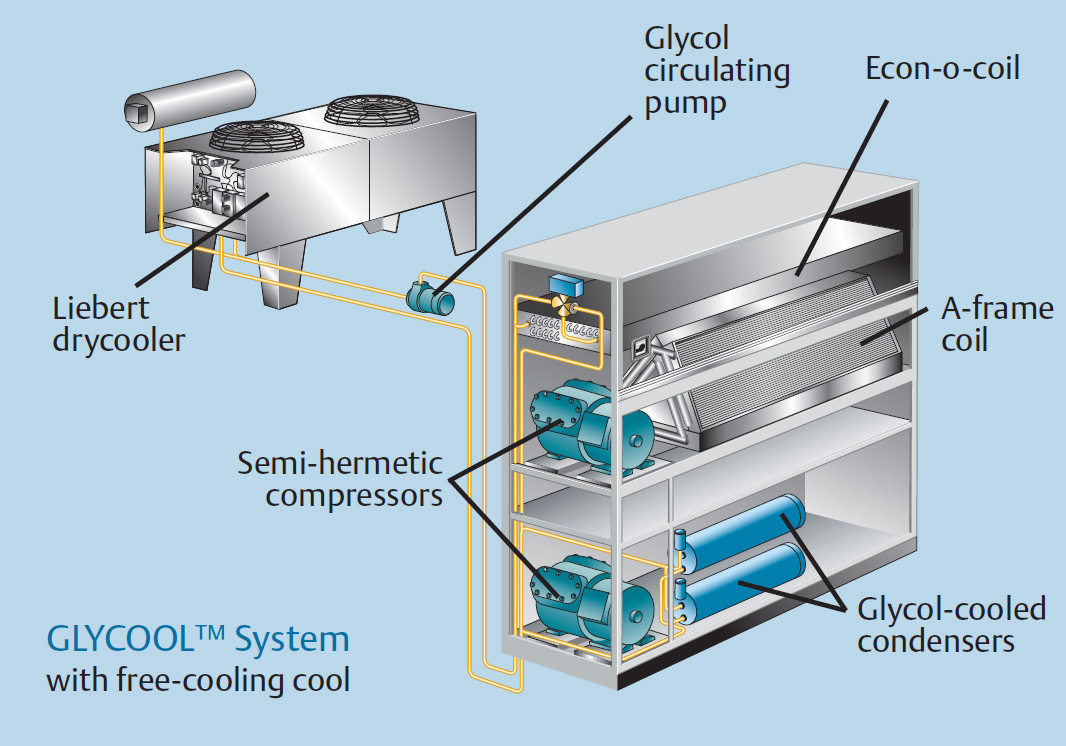
\includegraphics[width=0.75\linewidth]{glycool_liebert}
  \caption{Free cooling with Glycol-cooled DX CRAC (Liebert)}
  \label{fig:glycol-free-cooling}
\end{figure}

\begin{itemize}
\item Does not require CRAC to be near outside wall.
\item Outdoor air not introduced to data centre environment:
  \begin{itemize}
  \item Maintains air quality
  \item Easier to manage humidity in most cases
  \end{itemize}
\end{itemize}


%\subsection{Chiller bypass}

\bibliographystyle{plainnat}
\bibliography{bibliography}

\end{document}

